\begin{frame}{Hierarchical Attention Networks}
  \begin{columns}[T,onlytextwidth]
    \column{0.60\textwidth}
      \begin{itemize}\footnotesize\itemsep0.25em
        \item[\textcolor{red}{$\blacktriangleright$}] A \textbf{hierarchical attention network} (HAN) builds sentence vectors from words, then a document vector from sentences.
        \item[\textcolor{red}{$\blacktriangleright$}] \textbf{Word level.} A bidirectional GRU (covered earlier) reads sentence $i$ and returns an annotation $\mathbf{h}_{it}$ for each word $t$. Attention pools the words of the sentence:
          \[ \alpha_{it} = \frac{\exp(\mathbf{u}_{it}^\top \mathbf{u}_w)}{\sum_{t'} \exp(\mathbf{u}_{it'}^\top \mathbf{u}_w)}, \qquad \mathbf{s}_i = \sum_t \alpha_{it}\, \mathbf{h}_{it}. \]
          Here $\mathbf{u}_{it} = \tanh(W_w \mathbf{h}_{it} + \mathbf{b}_w)$, $\mathbf{u}_w$ is a learned query (``what is the informative word''), $\alpha_{it}$ the weight of word $t$ and $\mathbf{s}_i$ the sentence vector: additive attention (covered earlier) with a learned query instead of a decoder state.
        \item[\textcolor{red}{$\blacktriangleright$}] \textbf{Sentence level.} A second bidirectional GRU reads $\mathbf{s}_1, \mathbf{s}_2, \dots$ and returns $\mathbf{h}_i$. The same pooling with its own query $\mathbf{u}_s$ gives the document vector $\mathbf{v} = \sum_i \alpha_i \mathbf{h}_i$, and $\operatorname{softmax}(W_c \mathbf{v} + \mathbf{b}_c)$ predicts the class.
        \item[\textcolor{red}{$\blacktriangleright$}] Yelp 2015 accuracy (1.57M reviews, five ratings; Table~2): flat word-level CNN 61.5\%, HAN with uniform weights ($\mathbf{u}_w = \mathbf{u}_s = \mathbf{0}$) 69.9\%, full HAN 71.0\%. The hierarchy gives most of the gain.
      \end{itemize}
    \column{0.38\textwidth}
      \centering
      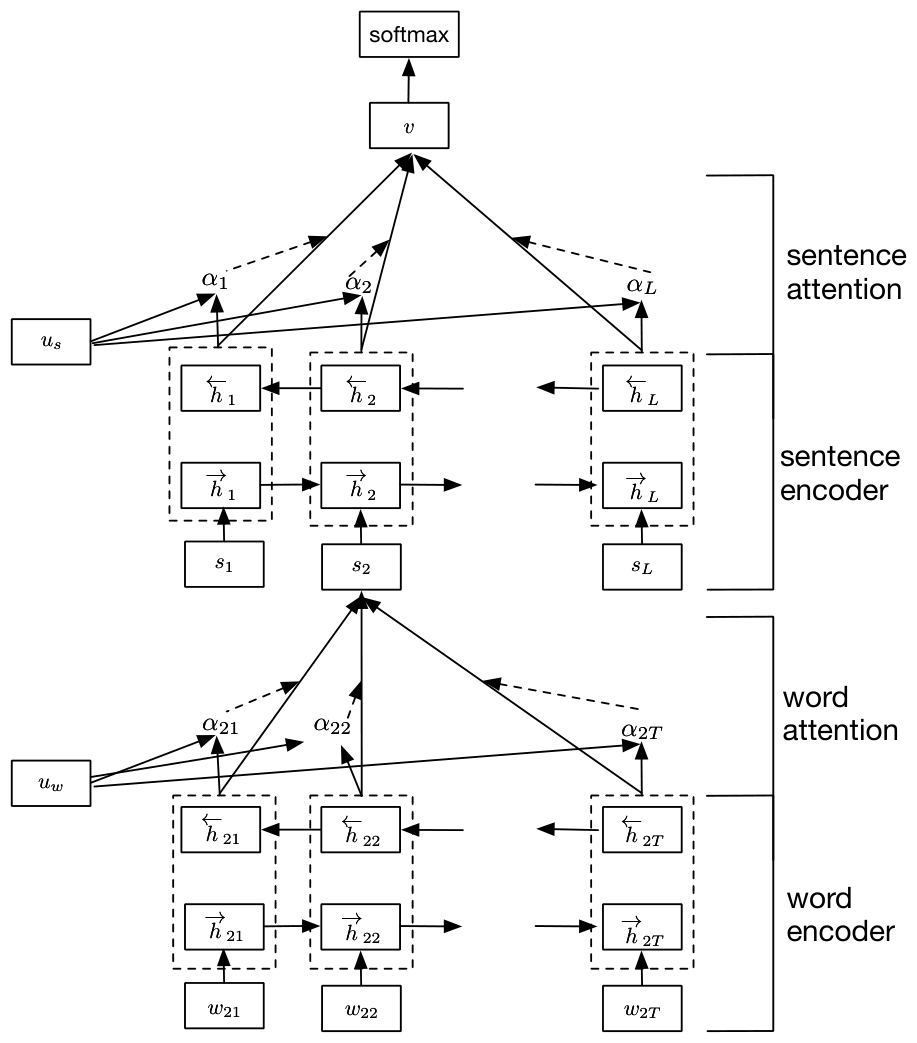
\includegraphics[width=\linewidth,height=0.64\textheight,keepaspectratio]{images/long-context/han_fig2_hierarchical_attention_network.png}\\[0.2em]
      {\scriptsize Yang et al., ``Hierarchical Attention Networks for Document Classification,'' NAACL 2016, \href{https://aclanthology.org/N16-1174/}{aclanthology.org/N16-1174}, Figure~2.\par}
  \end{columns}
\end{frame}

\begin{frame}{Two-Level Transformers for Long Documents}
  \begin{columns}[T,onlytextwidth]
    \column{0.58\textwidth}
      \begin{itemize}\footnotesize\itemsep0.25em
        \item[\textcolor{red}{$\blacktriangleright$}] Replace the GRUs with Transformers. Split the $n$ tokens into $n/s$ segments of $s$ tokens ($s$: segment length), attend fully inside each segment, then across one summary vector per segment. Scores per layer:
          \[ \tfrac{n}{s}\cdot s^2 + \big(\tfrac{n}{s}\big)^2 = ns + \big(\tfrac{n}{s}\big)^2 \quad \text{instead of } n^2. \]
        \item[\textcolor{red}{$\blacktriangleright$}] \textbf{Worked number:} $n = 16{,}384$ and $s = 128$ give $2{,}097{,}152 + 16{,}384 \approx 2.1$ million scores against $n^2 \approx 268$ million, a $127\times$ cut. The sum is smallest at $s = (2n)^{1/3}$, here $s = 32$ and 0.79 million scores.
        \item[\textcolor{red}{$\blacktriangleright$}] \textbf{Hi-Transformer} uses sentences as segments: a sentence Transformer over each sentence plus an appended [CLS] token, a document Transformer across the $n/s$ [CLS] vectors, then a second sentence Transformer that re-reads each sentence with its document-aware vector. With sentences of $s$ words and width $d$, the cost is $O(nsd + (n/s)^2 d)$ against $O(n^2 d)$.
        \item[\textcolor{red}{$\blacktriangleright$}] Words in different sentences meet only through summaries. Dropping the downward pass lowers accuracy on all three datasets tested, e.g.\ MIND news topics from 82.51\% to 81.92\% (Figure~2).
      \end{itemize}
    \column{0.40\textwidth}
      \centering
      \vspace{1.0em}
      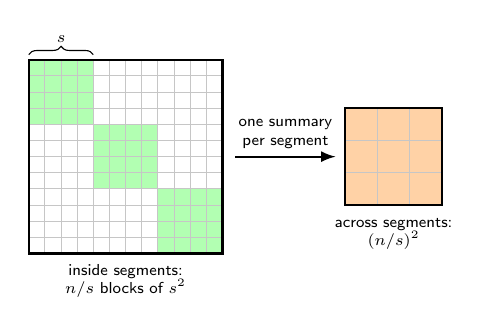
\begin{tikzpicture}[font=\sffamily\scriptsize, >=latex, scale=0.82,
          every node/.style={transform shape}]
        % 12 tokens in 3 segments of s = 4; cell 0.25 cm, row 0 at the top
        \foreach \k in {0,1,2} {
          \fill[green!30] (\k,{2-\k}) rectangle ({\k+1},{3-\k});
        }
        \draw[gray!45, step=0.25] (0,0) grid (3,3);
        \draw[thick] (0,0) rectangle (3,3);
        \draw[decorate, decoration={brace, amplitude=3pt}] (0,3.08) -- (1,3.08) node[midway, above=2pt] {$s$};
        \node[align=center] at (1.5,-0.42) {inside segments:\\ $n/s$ blocks of $s^2$};
        \fill[orange!35] (4.9,0.75) rectangle (6.4,2.25);
        \draw[gray!45, step=0.5, shift={(4.9,0.75)}] (0,0) grid (1.5,1.5);
        \draw[thick] (4.9,0.75) rectangle (6.4,2.25);
        \node[align=center] at (5.65,0.3) {across segments:\\ $(n/s)^2$};
        \draw[->, thick] (3.2,1.5) -- (4.75,1.5) node[midway, above, align=center] {one summary\\ per segment};
      \end{tikzpicture}\\[0.4em]
      {\scriptsize Shaded cells are the scores one layer computes for 12 tokens in segments of 4. Full attention would fill the whole square.\par}
      \vspace{0.6em}
      {\scriptsize Wu et al., ``Hi-Transformer: Hierarchical Interactive Transformer for Efficient and Effective Long Document Modeling,'' ACL 2021, \href{https://arxiv.org/abs/2106.01040v3}{arXiv:2106.01040v3}.\par}
  \end{columns}
\end{frame}

\begin{frame}{Longformer: Sliding, Dilated and Global Attention}
  \centering
  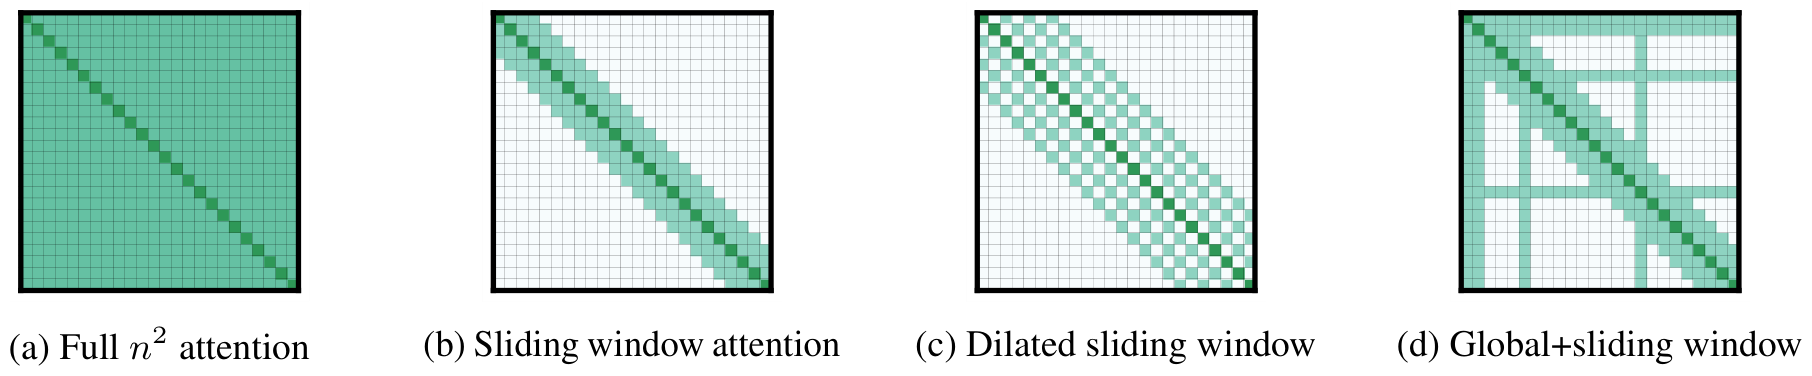
\includegraphics[width=\textwidth,height=0.30\textheight,keepaspectratio]{images/long-context/longformer_fig2_attention_patterns.png}\\[0.1em]
  {\scriptsize Beltagy et al., ``Longformer: The Long-Document Transformer,'' arXiv 2020, \href{https://arxiv.org/abs/2004.05150v2}{arXiv:2004.05150v2}, Figure~2.}\par
  \vspace{0.3em}
  \begin{columns}[T,onlytextwidth]
    \column{0.49\textwidth}
      \begin{itemize}\footnotesize\itemsep0.3em
        \item[\textcolor{red}{$\blacktriangleright$}] \textbf{(b) Sliding window} (covered earlier), here inside a bidirectional encoder: $w/2$ tokens on each side, cost $O(nw)$, receptive field $L \cdot w$ after $L$ layers.
        \item[\textcolor{red}{$\blacktriangleright$}] \textbf{(c) Dilated window:} attend to every $\delta$-th position, as a dilated convolution does (covered in the CV course). The receptive field grows to $L \cdot \delta \cdot w$ at the same cost. Heads can differ: undilated heads keep local detail while dilated heads reach far. The character-level model widens $w$ from lower to upper layers and dilates only 2 heads of the upper layers.
      \end{itemize}
    \column{0.49\textwidth}
      \begin{itemize}\footnotesize\itemsep0.3em
        \item[\textcolor{red}{$\blacktriangleright$}] \textbf{(d) Global attention} on a few positions chosen per task: [CLS] for classification, every question token for QA. It is symmetric: a global token attends to all $n$ tokens and all tokens attend to it. With $g$ global tokens there are about $n(w + 2g)$ scores, still linear in $n$.
        \item[\textcolor{red}{$\blacktriangleright$}] Global attention has its own projections $Q_g, K_g, V_g$, initialised as copies of the window projections $Q_s, K_s, V_s$. WikiHop dev accuracy after 5 fine-tuning epochs (Table~10): 73.8 with both, 72.2 without the separate projections, 65.5 with no global attention.
      \end{itemize}
  \end{columns}
\end{frame}

\begin{frame}{Longformer: Extending RoBERTa to 4,096 Tokens}
  \begin{columns}[T,onlytextwidth]
    \column{0.56\textwidth}
      \begin{itemize}\footnotesize\itemsep0.25em
        \item[\textcolor{red}{$\blacktriangleright$}] Longformer starts from the RoBERTa checkpoint and continues masked-language-model (MLM) training. Every layer uses a window of $w = 512$, so each token does the same attention work as in 512-token RoBERTa.
        \item[\textcolor{red}{$\blacktriangleright$}] RoBERTa learned only 512 absolute position embeddings; all 4,096 positions start as 8 back-to-back copies of them. Several BERT heads attend mainly to the previous or next token, so the copies keep that local structure except at the 7 seams. LED, the encoder--decoder variant, stretches BART from 1K to 16K positions the same way.
        \item[\textcolor{red}{$\blacktriangleright$}] MLM bits per character, base size (Table~5): RoBERTa at 512 tokens 1.846; Longformer at 4,096 with random new positions 10.299, with copies 1.957, after 2K updates 1.753, after 65K updates 1.705.
        \item[\textcolor{red}{$\blacktriangleright$}] The RoBERTa baseline encodes 512-token pieces separately and concatenates the outputs. Longformer reads up to 4,096 tokens in one pass, with global attention on the question or on [CLS]. The largest gain is on Hyperpartisan: 645 news articles averaging 705 wordpieces.
      \end{itemize}
    \column{0.42\textwidth}
      \centering
      \vspace{0.6em}
      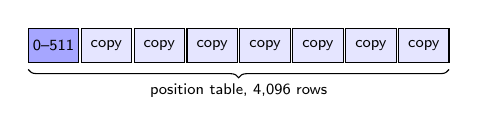
\begin{tikzpicture}[font=\sffamily\scriptsize, scale=0.8,
          every node/.style={transform shape},
          posbox/.style={draw, minimum width=0.8cm, minimum height=0.55cm, inner sep=0pt}]
        \node[posbox, fill=blue!35] at (0,0) {0--511};
        \foreach \i in {1,...,7} {
          \node[posbox, fill=blue!10] at ({0.84*\i},0) {copy};
        }
        \draw[decorate, decoration={brace, amplitude=3pt, mirror}] (-0.4,-0.38) -- (6.28,-0.38) node[midway, below=3pt] {position table, 4,096 rows};
      \end{tikzpicture}\\[0.3em]
      {\scriptsize Initial position table: RoBERTa's 512 learned rows, then 7 copies.\par}
      \vspace{0.8em}
      {\scriptsize\setlength{\tabcolsep}{4pt}
      \begin{tabular}{lcc}
        \toprule
        \textbf{Task (metric)} & \textbf{RoBERTa} & \textbf{Longformer} \\
        \midrule
        WikiHop (acc.) & 72.4 & 75.0 \\
        TriviaQA (F1) & 74.3 & 75.2 \\
        HotpotQA (joint F1) & 63.5 & 64.4 \\
        OntoNotes (avg.\ F1) & 78.4 & 78.6 \\
        IMDB (acc.) & 95.3 & 95.7 \\
        Hyperpartisan (F1) & 87.4 & 94.8 \\
        \bottomrule
      \end{tabular}\par}
      \vspace{0.3em}
      {\scriptsize Base models, development sets. Beltagy et al., \href{https://arxiv.org/abs/2004.05150v2}{arXiv:2004.05150v2}, Tables~5--7.\par}
  \end{columns}
\end{frame}

\begin{frame}{BigBird: Random, Window and Global Attention}
  \centering
  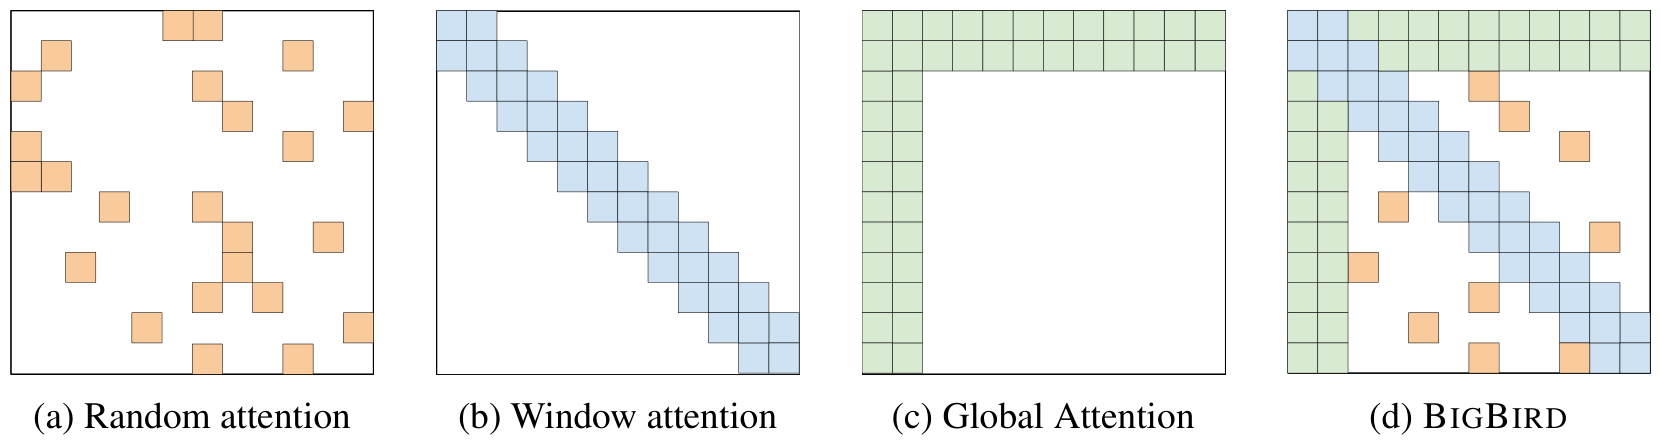
\includegraphics[width=\textwidth,height=0.21\textheight,keepaspectratio]{images/long-context/bigbird_fig1_attention_components.png}\\[0.1em]
  {\scriptsize Zaheer et al., ``Big Bird: Transformers for Longer Sequences,'' NeurIPS 2020, \href{https://arxiv.org/abs/2007.14062v2}{arXiv:2007.14062v2}, Figure~1.}\par
  \vspace{0.1em}
  \begin{columns}[T,onlytextwidth]
    \column{0.49\textwidth}
      \begin{itemize}\footnotesize\itemsep0.25em
        \item[\textcolor{red}{$\blacktriangleright$}] As a graph, query $i$ reads key $j$ only along an edge, and full attention is the complete graph. BigBird keeps \textbf{(a)} $r$ random keys per query, \textbf{(b)} a window of $w$ neighbours, \textbf{(c)} $g$ global tokens joined to every token both ways.
        \item[\textcolor{red}{$\blacktriangleright$}] Random graphs with $\tilde{O}(n)$ edges ($\tilde{O}$ hides log factors) have $O(\log n)$ shortest paths, so information mixes fast.
        \item[\textcolor{red}{$\blacktriangleright$}] BigBird-ITC (internal transformer construction: some existing tokens are made global) base uses blocks of $b = 64$ with $g = 2b$, $w = 3b$, $r = 3b$: each non-global query reads $128 + 192 + 192 = 512$ keys, as in 512-token BERT, but $n = 4{,}096$ (Table~8), 8$\times$ longer on similar 16\,GB chips.
      \end{itemize}
    \column{0.49\textwidth}
      \begin{itemize}\footnotesize\itemsep0.25em
        \item[\textcolor{red}{$\blacktriangleright$}] \textbf{Universal approximation} (Theorem~1): with a star in the graph, one global token joined to all, sparse attention approximates any continuous sequence-to-sequence function. A sparse encoder--decoder is Turing complete, assuming arbitrary precision as for full attention.
        \item[\textcolor{red}{$\blacktriangleright$}] \textbf{No free lunch} (Proposition~1): finding each vector's farthest vector takes one full-attention layer, but $\tilde{\Omega}(n^{1-o(1)})$ layers for any sparse pattern with $\tilde{O}(n)$ edges.
        \item[\textcolor{red}{$\blacktriangleright$}] Without global tokens, at 512 tokens: SQuAD 85.1 against 88.5 for BERT (Table~1). At 4,096 tokens: TriviaQA dev F1 79.5, against 75.2 for Longformer and 74.3 for RoBERTa (Table~2).
      \end{itemize}
  \end{columns}
\end{frame}

\begin{frame}{H-Transformer-1D: Fine Near, Coarse Far}
  \begin{columns}[T,onlytextwidth]
    \column{0.53\textwidth}
      \begin{itemize}\footnotesize\itemsep0.25em
        \item[\textcolor{red}{$\blacktriangleright$}] An LSTM language model uses about 200 tokens of context but ignores word order beyond the last 50, keeping the distant past ``only as a rough semantic field or topic.''
        \item[\textcolor{red}{$\blacktriangleright$}] H-Transformer-1D builds this into attention with a \textbf{hierarchical matrix} (H-matrix) from numerical analysis: exact blocks near the diagonal, low-rank blocks farther away, larger with distance.
        \item[\textcolor{red}{$\blacktriangleright$}] Average adjacent pairs of queries and keys (sum the values) to get $n/2, n/4, \dots$ coarse tokens over $\log_2(n/b)$ levels. At each level a block of $b$ tokens attends only to neighbouring blocks, so a level-$l$ score stands for $2^l \times 2^l$ token pairs. Every block is $b \times b$, which suits dense GPU kernels; building and applying the matrix each take about $5nbd$ operations, linear in $n$.
        \item[\textcolor{red}{$\blacktriangleright$}] One Billion Word perplexity: 20.25 at 144M parameters, against 21.8 for Transformer-XL (later in this lecture) at 800M (Table~2).
      \end{itemize}
      \vspace{0.1em}
      {\scriptsize Khandelwal et al., ``Sharp Nearby, Fuzzy Far Away: How Neural Language Models Use Context,'' ACL 2018, \href{https://arxiv.org/abs/1805.04623v1}{arXiv:1805.04623v1}.\par}
    \column{0.45\textwidth}
      \centering
      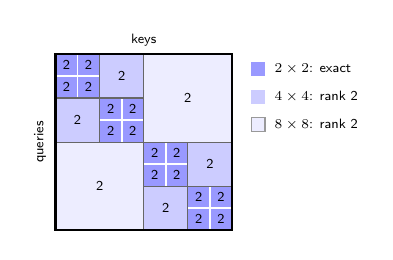
\begin{tikzpicture}[font=\sffamily\scriptsize, scale=0.7,
          every node/.style={transform shape}]
        % 16 x 16 attention matrix, cell 0.2 cm, row 0 at the top
        \fill[blue!7] (1.6,1.6) rectangle (3.2,3.2);
        \fill[blue!7] (0,0) rectangle (1.6,1.6);
        \fill[blue!20] (0.8,2.4) rectangle (1.6,3.2);
        \fill[blue!20] (0,1.6) rectangle (0.8,2.4);
        \fill[blue!20] (2.4,0.8) rectangle (3.2,1.6);
        \fill[blue!20] (1.6,0) rectangle (2.4,0.8);
        \foreach \k in {0,1,2,3} {
          \fill[blue!40] ({0.8*\k},{2.4-0.8*\k}) rectangle ({0.8*\k+0.8},{3.2-0.8*\k});
          \draw[white, line width=0.6pt] ({0.8*\k+0.4},{2.4-0.8*\k}) -- ++(0,0.8);
          \draw[white, line width=0.6pt] ({0.8*\k},{2.8-0.8*\k}) -- ++(0.8,0);
          \foreach \dx in {0.2,0.6} {
            \foreach \dy in {0.2,0.6} {
              \node at ({0.8*\k+\dx},{2.4-0.8*\k+\dy}) {2};
            }
          }
        }
        \draw[black!60] (0,1.6) -- (3.2,1.6) (1.6,0) -- (1.6,3.2);
        \draw[black!60] (0,2.4) -- (1.6,2.4) (0.8,1.6) -- (0.8,3.2);
        \draw[black!60] (1.6,0.8) -- (3.2,0.8) (2.4,0) -- (2.4,1.6);
        \draw[thick] (0,0) rectangle (3.2,3.2);
        \node at (2.4,2.4) {2};
        \node at (0.8,0.8) {2};
        \node at (1.2,2.8) {2};
        \node at (0.4,2.0) {2};
        \node at (2.8,1.2) {2};
        \node at (2.0,0.4) {2};
        \node at (1.6,3.45) {keys};
        \node[rotate=90] at (-0.28,1.6) {queries};
        \fill[blue!40] (3.55,2.8) rectangle (3.8,3.05);
        \node[anchor=west] at (3.85,2.925) {$2\times2$: exact};
        \fill[blue!20] (3.55,2.3) rectangle (3.8,2.55);
        \node[anchor=west] at (3.85,2.425) {$4\times4$: rank 2};
        \draw[black!40, fill=blue!7] (3.55,1.8) rectangle (3.8,2.05);
        \node[anchor=west] at (3.85,1.925) {$8\times8$: rank 2};
      \end{tikzpicture}\\[0.1em]
      {\scriptsize Ranks for 16 tokens, redrawn after Zhu \& Soricut, ``H-Transformer-1D: Fast One-Dimensional Hierarchical Attention for Sequences,'' ACL 2021, \href{https://arxiv.org/abs/2107.11906v1}{arXiv:2107.11906v1}, Eq.~(20).\par}
      \vspace{0.4em}
      {\scriptsize\setlength{\tabcolsep}{2.5pt}
      \begin{tabular}{lcccc}
        \toprule
        \textbf{LRA accuracy} & \textbf{ListOps} & \textbf{Text} & \textbf{Pathfinder} & \textbf{Avg.} \\
        \midrule
        Transformer & 36.37 & 64.27 & 71.40 & 54.39 \\
        BigBird & 36.05 & 64.02 & 74.87 & 55.01 \\
        H-Transformer-1D & 49.53 & 78.69 & 68.78 & 61.41 \\
        \bottomrule
      \end{tabular}\par}
      \vspace{0.2em}
      {\scriptsize Long Range Arena (LRA): six classification tasks on 1K--16K tokens, such as ListOps (nested arithmetic) and Pathfinder (do two circles connect?). Avg.\ covers five tasks, two not shown. Every model here fails Path-X, which S4 (covered earlier) later solved. Table~1.\par}
  \end{columns}
\end{frame}

\begin{frame}{Fixed Patterns Compared}
  \centering
  {\scriptsize
  \setlength{\tabcolsep}{4pt}
  \begin{tabular}{>{\raggedright\arraybackslash}p{2.6cm} >{\raggedright\arraybackslash}p{3.0cm} >{\raggedright\arraybackslash}p{1.8cm} >{\raggedright\arraybackslash}p{2.5cm} >{\raggedright\arraybackslash}p{2.5cm}}
    \toprule
    \textbf{Pattern} & \textbf{Who attends to whom} & \textbf{Scores per layer} & \textbf{What is lost} & \textbf{Examples} \\
    \midrule
    Sliding window (covered earlier) & each token reads its $w$ nearest tokens & $nw$ & links beyond $w$ need many layers & Mistral~7B, Gemma~2/3 local layers \\
    \addlinespace[0.1em]
    Swin windows (covered in the CV course) & local windows, shifted in alternate layers & linear in patches & far patches interact only over depth & Swin Transformer \\
    \addlinespace[0.1em]
    Two-level segments & inside each segment, then across summaries & $ns + (n/s)^2$ & token links across segments & HAN, HIBERT, Hi-Transformer \\
    \addlinespace[0.1em]
    Window, dilation, global & window; dilated heads; $g$ global tokens & $\approx n(w + 2g)$ & global positions chosen by hand per task & Longformer, LED \\
    \addlinespace[0.1em]
    Window, random, global & window; $r$ random keys; $g$ global tokens & $\approx n(w + r + 2g)$ & some tasks need far more layers & BigBird \\
    \addlinespace[0.1em]
    Pooled hierarchy (H-matrix) & exact near blocks; coarser blocks farther away & $\approx 5nb$ & far detail averaged away & H-Transformer-1D \\
    \addlinespace[0.1em]
    Byte patches (covered earlier) & local byte models; a global model over patches & quadratic in patches & detail inside a patch compressed & MEGABYTE (fixed stride), BLT \\
    \bottomrule
  \end{tabular}\par}
  \vspace{0.3em}
  \begin{itemize}\footnotesize
    \item[\textcolor{red}{$\blacktriangleright$}] In every row, the keys a query may read are fixed before the query is compared with any key. The next part of this lecture lets each query choose which blocks to read.
  \end{itemize}
\end{frame}
